\chapter{Systemtechnische Lösung}
\label{chapter:Pflichtenheft-SystemtechnischeLoesung}

\section{Lösungsansatz}
\label{section:Pflichtenheft-SystemtechnischeLoesung-Loesungsansatz}

Der erste Schritt ist zu klären, wie die Tabelle im Speicher gespeichert werden soll. Dabei gilt zu beachten, dass unbegrenzt Speicher vorhanden ist und keine Bewertung hinsichtlich des Speichers getroffen wird.

\subsection{Ansatz 1}
Man speichert die Kanalnummer in Register x und die herausgefundene Anzahl Datenbits, die zu dieser Kanalnummer gehören, in Register x+1.

Vorteile:
\begin{itemize}
    \item Man findet sehr schnell zu einer Kanalnummer die entsprechende Anzahl.
    \item Geringer Speicherverbrauch.
\end{itemize}

Nachteile:
\begin{itemize}
    \item Die Kanalnummern werden sehr langsam gefunden, es sei denn man sortiert sie.
    \item Wenn man die Kanalnummern sortiert, muss man die höheren nach hinten verschieben.
\end{itemize}

\subsection{Ansatz 2}
Man speichert in der Speicherzelle mit der Kanalnummer (plus einem Offset, damit das Datenfeld nicht überschrieben wird) als Adresse die herausgefundene Anzahl Datenbits, die zu dieser Kanalnummer gehören.

Vorteile:
\begin{itemize}
    \item Sehr schnelle Bestimmung der Speicheradresse, an der die gewünschte Anzahl steht.
    \item Keine Sortierung notwendig.
    \item Reduzierung des Nettospeicherverbrauchs.
\end{itemize}

Nachteile:
\begin{itemize}
    \item Hoher Bruttospeicherverbrauch, da viele mögliche Nummern unnutzbaren Speicher darstellen.
    \item Schlecht "`per Auge"' ablesbar, weil man die Adresse berechnen muss.
\end{itemize}

Nach dem Beispiel aus \autoref{chapter:Pflichtenheft-Sollzustand} ergäbe sich folgende Tabelle:

\begin{center}
    \begin{tabular}{|r|r|l|}
        \hline
        Kanalnr. & Anzahl & Speicheradresse \\
        \hline
        \hline
        243 & 9 & Offset + 0xF3 \\
        \hline
        3727 & 4 & Offset + 0xE8F \\
        \hline
    \end{tabular}
\end{center}

Wir haben uns wegen der sehr umständlichen Speicheroperationen gegen den ersten Ansatz entschieden.

Im Allgemeinen arbeitet der Algorithmus wie folgt: Die Daten können aus dem Speicher nur blockweise gelesen werden. Deshalb wird in dem Register "`Blockspeicher"' immer der aktuelle Block gespeichert und in ein weiteres Register (Zwischenspeicher) geshiftet, in dem man die Daten bitweise prüfen kann.

Die Daten werden dann in einer Schleife in "`Blockspeicher"' eingelesen und durch eine weitere Schleife bitweise verarbeitet. In dieser zweiten Schleife wird entweder, wenn man an den Anfang eines Headers angekommen ist, die neue Kanalnummer gespeichert und an den Anfang des Datenteils gesprungen oder der Speicherblock inkrementiert, der die Anzahl Datenbits enthält.

Die Tabelle selber wird, wie bereits angedeutet, so gespeichert, dass die Speicheradresse äquivalent zur Kanalnummer ist (allerdings einen Offset hat). Der Offset entspricht dabei genau der Speicheradresse, die auf die erste freie Speicherzelle nach dem Datenteil zeigt.

Die Implementierung ist abstrahiert als Flussdiagramm visualisiert (siehe \autoref{figure:Pflichtenheft-SystemtechnischeLoesung-Loesungsansatz-Algorithmus}).

\begin{figure}[htb]
    \centering
    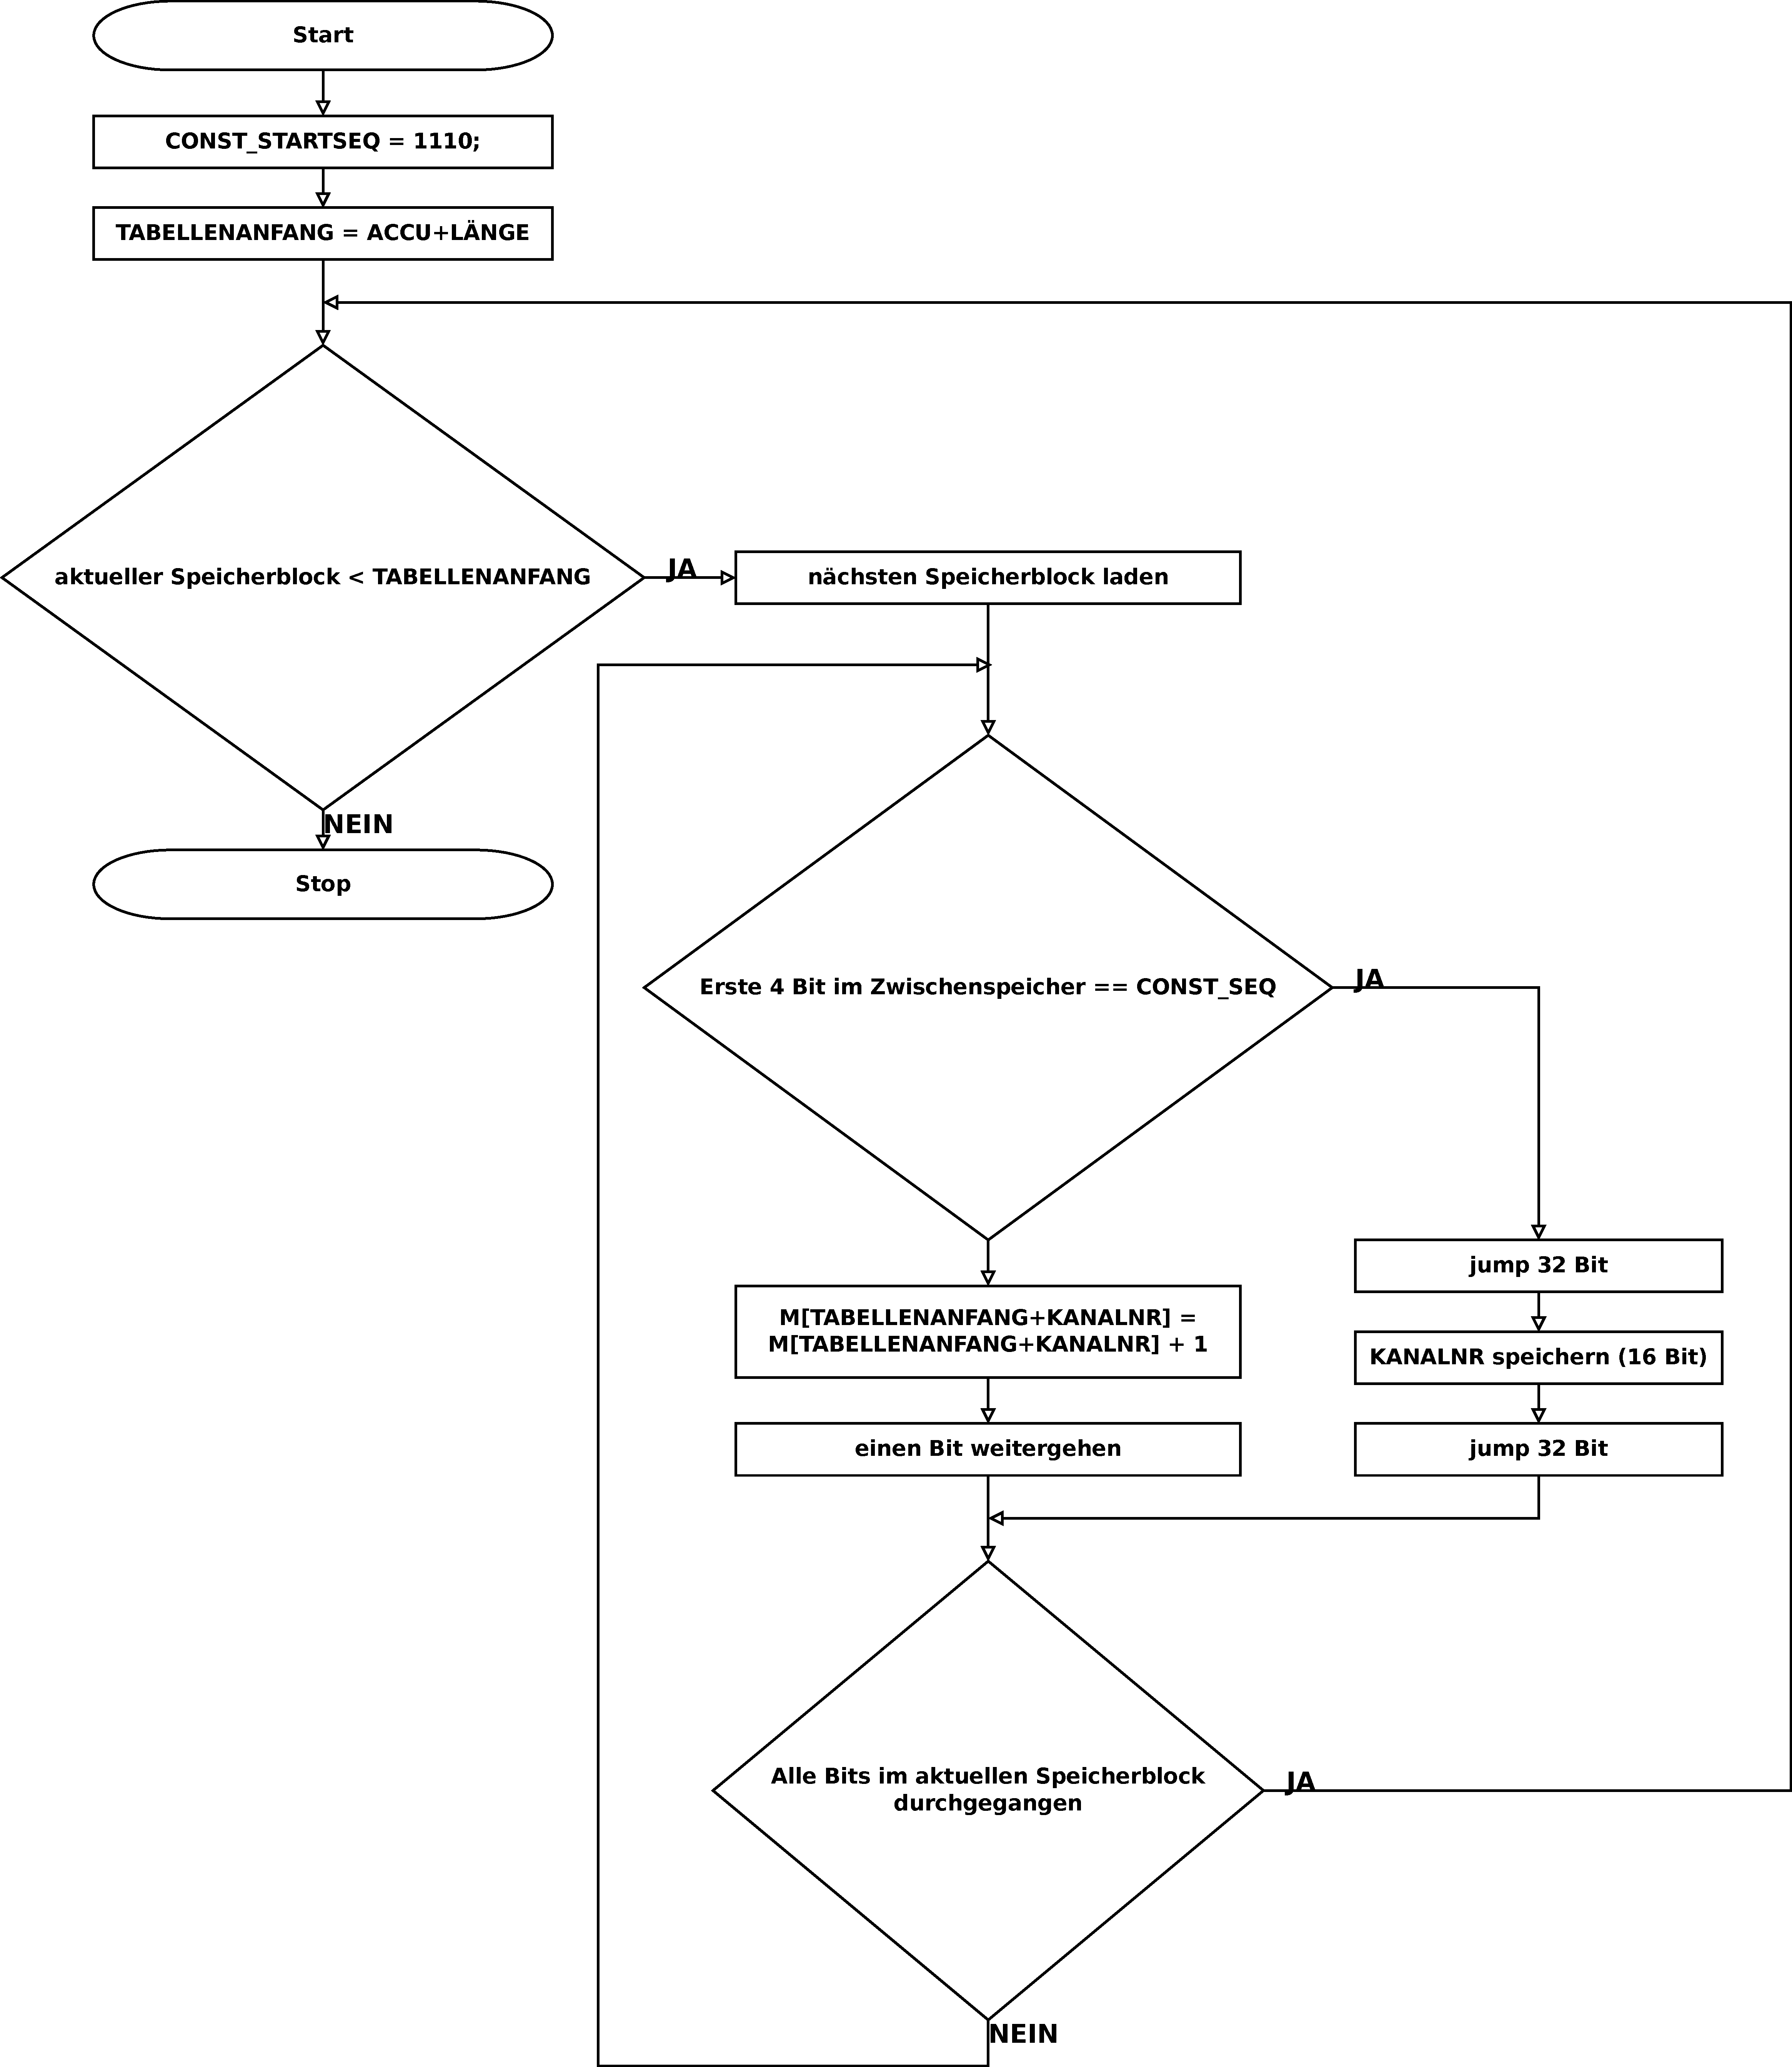
\includegraphics[width=\textwidth]{pflichtenheft/res/algorithmus.pdf}
    \caption{Schematischer Aufbau des Algorithmus}
    \label{figure:Pflichtenheft-SystemtechnischeLoesung-Loesungsansatz-Algorithmus}
\end{figure}

\clearpage

Es folgen noch einige Erläuterungen zu einzelnen Funktionen im Flussdiagramm.

\begin{description}
    \item[{Nächsten Speicherblock laden}] 32 Bit aus dem Speicher auslesen und in Blockspeicher speichern.
    
    \item[{ein Bit weitergehen}] Zwischenspeicher shiften und aus dem Blockspeicher ein Bit nachladen.
    
    \item[{jump 32 Bit}] Lade nächsten Block in Blockspeicher und shifte dort genauso viele Bits, wie man im aktuellen Speicherblock geshiftet hat. Im Zwischenspeicher befinden sich dann 32 neue Bits.
    
    \item[{KANALNR speichern}] Zwischenspeicher sechszehnmal shiften und die geshifteten Bits im Register "KANALNR" speichern
    
    \item[{M[TABELLENANFANG + KANALNR] = M[TABELLENANFANG + KANALNR] + 1}] Inkrementiert den Inhalt der Speicherzelle, in dem die Anzahl der Datenbits für die aktuelle Kanalnummer gespeichert wird.
\end{description}


\section{Gliederung}
\label{section:Pflichtenheft-SystemtechnischeLoesung-Gliederung}

Nach Auftragserteilung wird die Abarbeitung des Projekts in folgenden Schritten stattfinden:

\subsection{Algorithmus ausarbeiten}
Der Algorithmus wird auf Sprachlevel der Minimax"=Maschine ausgearbeitet und in RT"=Notation verfasst. Dieser Aufgabe sind \emph{Gerion Entrup} und \emph{Sergej Wildemann} zugewiesen.

\subsection{Erweiterung der Minimax"=Maschine}
Die erforderlichen Erweiterungen der Minimax"=Maschine werden vorgenommen. Dazu werden notwendige Konfigurationsdateien erstellt und dokumentiert. Diese Dateien sind im Anschluss mit Minimalbeispielen zu testen. Auch dieser Abschnitt wird von \emph{Gerion Entrup} und \emph{Sergej Wildemann} übernommen.

\subsection{Steuertabelle erstellen}
Der Pseudocode in RT"=Notation wird in Maschinencode für die Minimax"=Maschine umgewandelt. Im Anschluss muss dieser ausgiebig u.\,a. mit den gegebenen Benchmarkdateien getestet und ggf. überarbeitet werden. Dieser Teil wird von \emph{Martin Matthaei} durchgeführt.

\subsection{Dokumentation erstellen}
Der Arbeitsfortschritt wird in einer Dokumentation (\autoref{part:Dokumentation}) protokolliert. Ebenfalls enthalten sind Kommentare und abschließende Bewertung. Diese Aufgabe wird parallel zu den anderen Schritten von \emph{Sven Karsten Greiner} durchgeführt und abschließend überprüft.

\subsection{Fertigstellung}
Der Auftrag ist bis zum \emph{24.01.2012 um 11 Uhr} zu erfüllen (siehe \autoref{subsection:Pflichtenheft-Einfuehrung-Projektumfeld-Ablauf}), eine vorzeitige Abgabe ist jedoch möglich. Sollten unerwartet Verzögerungen eintreten, ist der Auftraggeber umgehend zu informieren. Sollte es zu verstärktem Personalausfall kommen, muss der o.\,g. Ablauf abgeändert werden. Es ist jedoch nicht auszuschließen, dass ggf. einige Teile nicht fertiggestellt werden können. In diesem Fall ist es notwendig, in Zusammenarbeit mit dem Auftraggeber nach Alternativen zu suchen.

\subsection{Benötigte Ressourcen}
Für dieses Projekt werden keine besonderen Ressourcen in Anspruch genommen. Der Arbeitsaufwand wird mit 16 Stunden pro Person geschätzt und wird im Rahmen des Informatik"=Studiums an der Leibniz Universität Hannover abgeleistet.

Zum Personal siehe auch \autoref{subsection:Pflichtenheft-Einfuehrung-Projektumfeld-Personal}.

\pagebreak

\section[Regulärer Betrieb]{Regulärer Betrieb\footnote{Die folgenden beiden Abschnitte beziehen sich auf den zuvor gewählten Ansatz}}
\label{section:Pflichtenheft-SystemtechnischeLoesung-regulaer}

Nach Aufruf des Alorithmus mit korrekten Startparametern (siehe \autoref{chapter:Pflichtenheft-Sollzustand}), läuft dieser solange, bis er nach Erreichen der gegebenen Länge des Datenfelds terminiert. Im Hauptspeicher liegt dann eine Tabelle der Kanalnummern und ihrer jeweiligen Datenlänge vor.


\section{Irregulärer Betrieb}
\label{section:Pflichtenheft-SystemtechnischeLoesung-irregulaer}

Eine Reihe von Ereignissen kann zu einem fehlerhaften Verhalten des Algorithmus führen.

\subsection{Fehlerhafte Startparameter}
\label{subsection:Pflichtenheft-SystemtechnischeLoesung-irregulaer-startparameter}

Es kann sein, dass der übergebene Parameter nicht den korrekten Beginn des Datenfeldes beschreibt. In diesem Fall ist nicht vorherzusehen, wie sich der Algorithmus verhält. Man kann allerdings überprüfen, ob der Beginn mit dem Startcode \texttt{1110} beginnt und diesen Fehlerfall somit weitgehend vermeiden.

Falls die angegebene Länge nicht zu den Daten im Hauptspeicher passt, wird entweder ein Teil der Daten vernachlässigt oder undefinierter Speicherinhalt gelesen und dem Ergebnis hinzugefügt. Dies verfälscht zwar das Ergebnis, lässt den Algorithmus jedoch korrekt terminieren. Sofern der Code \texttt{1110} im undefinierten Teil vorkommt, werden u.\,U. weitere falsche Kanäle hinzugefügt oder bereits vorhandene überschrieben (siehe \autoref{subsection:Pflichtenheft-SystemtechnischeLoesung-irregulaer-syntax}).

\subsection{Fehlerhafte Datensyntax}
\label{subsection:Pflichtenheft-SystemtechnischeLoesung-irregulaer-syntax}

Jedes Paket beginnt mit dem Muster \texttt{1110} (vgl. \autoref{chapter:Pflichtenheft-Sollzustand}). Sollte dieses Muster unerwartet \emph{nicht} als Beginn eines Pakets auftreten, arbeitet der Algorithmus vorrübergehend fehlerhaft weiter, bis er wieder auf ein neues Paket mit korrekter Syntax trifft.

Laut Definition der Daten kann \texttt{1110} jedoch nicht an einer solchen falschen Stelle auftreten. Einzige Möglichkeit wäre demzufolge ein fehlerhafter Einsatz des Algorithmus oder eine Beschädigung des Datenfeldes.

\subsection{Modifikation des Datenfeldes während der Laufzeit}
\label{subsection:Pflichtenheft-SystemtechnischeLoesung-irregulaer-moddatenfeld}

Findet während der Laufzeit eine Modifikation des Datenfeldes statt, welches bereits abgearbeitet wurde, so ändert dies das Ergebnis nicht. Eine Modifikation des kommenden Teils führt zu einem verfälschtem Ergebnis (vgl. \autoref{subsection:Pflichtenheft-SystemtechnischeLoesung-irregulaer-startparameter}).

\subsection{Modifikation des Tabellenteils während der Laufzeit}
\label{subsection:Pflichtenheft-SystemtechnischeLoesung-irregulaer-modtabelle}

Eine Modifikation der Ergebnistabelle während der Laufzeit führt zu fehlerhaften Datenlängen in der Tabelle.
